% !TeX encoding = UTF-8
% !TeX program = xelatex
% !TeX spellcheck = en_US

\documentclass[a4paper]{article}
\usepackage{amsmath}
\usepackage[english]{babel}
\usepackage[UTF8]{ctex}
\usepackage{unicode-math}
\usepackage{caption}
\usepackage{booktabs}
\usepackage{xcolor}
\usepackage{array}
\usepackage{listings}
\usepackage{hypdoc}
\usepackage[left=0.50in,right=0.50in,top=1.0in,bottom=1.0in,paperheight=11in,paperwidth=8.5in]{geometry}
\usepackage{endnotes}
\usepackage{graphicx}
\usepackage{multicol}
\usepackage{float}
\usepackage{blindtext}
\usepackage{listings}
\usepackage{xcolor}
\lstset{frame=tb,
  language=Java,
  aboveskip=3mm,
  belowskip=3mm,
  showstringspaces=false,
  columns=flexible,
  basicstyle={\small\ttfamily},
  numbers=none,
  numberstyle=\tiny\color{gray},
  keywordstyle=\color{blue},
  commentstyle=\color{green},
  stringstyle=\color{purple},
  breaklines=true,
  breakatwhitespace=true,
  tabsize=3
}
\setlength{\columnsep}{1cm}
\title{Lab report:\\ Measuring Young's modulus and Poisson's ratio of a metal wire}
\author{TiankaiMa PB21000030}
\date{\today}
\begin{document}
\begin{multicols*}{2}
    \maketitle
    \begin{abstract}
        Both Young's modulus and Poisson's ratio reflect important properties of a material. In this experiment, we take a metal wire as a target to present a way to measure both quantities.
        \par
        \textbf{Keywords:} Young's modulus, Poisson's ratio
    \end{abstract}
    \section*{Introduction}

    Young's modulus is an important mechanical parameter of a material that reflects the amount of resistance to deformation. Stress is defined as the ratio of the tensile force $F$ to the original cross-section A, and the ratio of $\Delta L$ to the original length $L$ is defined as the longitudinal line strain, In the elastic range, this could be described as a linear relationship named Hooke's Law:
    \begin{equation}
        \dfrac{F}{A} = E\cdot\dfrac{\Delta L}{L}
    \end{equation}

    Only longitudinal strain in the material is considered in the equation above, we define the transverse line strain as the ratio of the transverse variation $\Delta d$ to the transverse length $d$. Experiment shows that they follow a linear relationship:
    \begin{equation}
        \dfrac{\Delta d}{d} = -\mu\cdot\dfrac{\Delta L}{L}
    \end{equation}

    The negative sign shows that longitudinal stretching leads to transverse shrinkage and vice versa.

    Notice that the $\Delta d$ is way too small to measure, we can measure the resistivity $\rho\propto 1/d^2$.

    In this experiment, we also need to use an unbalanced bridge to measure the small change in resistance, illustrated as follows:

    \begin{figure}[H]
        \centering
        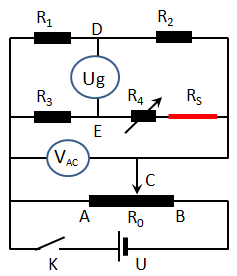
\includegraphics[width=0.5\linewidth]{./img/Fig.1.png}
        \caption{unbalanced bridge used to measure resistance}
        \label{fig:figure1}
    \end{figure}

    When $U_g$ is balanced out, the bridge follows that: $R_1 / R_2 = R_3 /(R_4 + R_s)$, where the $R_s$ is changing when the wire stretches. We can use this equation to calculate the resistance $R_s$: When given a change of $\Delta R_s\leq(R_4 + R_s)\cdot1\%$, the bridge approximately follows:

    \begin{equation}
        U_g \approx \frac{U_{AC}}{4}\cdot\frac{\Delta R_s}{R_4 + R_s}
    \end{equation}

    \section*{Materials}
    Connect the circuit as the unbalanced bridge shows, where $R_1 = R_2 = R_3 = 51.00\Omega$, and connect $R_4$ into a resistance box.

    Mesaure both $U_g$ and $U_{AC}$, keep $U_{AC}\sim (0.3V, 0.5V)$, change $R_4$ to make the bridge balanced (when $\mid U_g\mid < 0.020mV$ is considered balanced).

    To measure Young's modulus, the change in length also needs to be measured with a reading microscope pointing at the solder joint $\mathbb{W}$.

    \section*{Results}
    \begin{equation}
        \begin{aligned}
            D &= 0.2mm \\
            R_4 + R_s &= 51.00\Omega\\
            L_1 + L_2 &= 121.2cm\\
            L_2 &= 26.8cm\\
            V_{AC} &= 0.400V\\
            R_4 &= 14.97\Omega\\
        \end{aligned}
    \end{equation}
    Images are attached in a separate paper.
    \section*{Discussion}
    \begin{equation}
        \begin{aligned}
            R_s &=\rho \dfrac{L}{A}\\
            \dfrac{\Delta d}{d} &= -\mu\cdot\dfrac{\Delta L}{L}\\
            \dfrac{\Delta R_s}{R_s} &= (1+2\mu)\dfrac{\Delta L}{L}\\
            U_g &= \dfrac{U_{AC}}{4}\cdot\dfrac{\Delta R_s}{R_4 + R_s}\\
            \Delta R_s &= 4(R_4 + R_s)\cdot\dfrac{U_g}{U_{AC}}\\
        \end{aligned}
    \end{equation}

    For that we can conclude:
    \begin{equation}
        U_g = \dfrac{U_{AC}}{4}\cdot\dfrac{R_s\cdot(1+2\mu)\cdot\dfrac{\Delta L}{L}}{R_4 + R_s} = \dfrac{U_{AC}R_s(1+2\mu)}{4(R_4 + R_s)}\Delta L
    \end{equation}

    Young's modulus:
    \begin{equation}
        E = \dfrac{\pi R^2 k_{\Delta L \sim m}}{g(L_1 + L_2)} = 2.288\times 10^{-11} E/Pa
    \end{equation}
    Poisson's ratio:
    \begin{equation}
        \mu = \frac 12 (\dfrac{4k(R_s + R_4)}{R_s U_{AC}} - 1) = 0.237
    \end{equation}

    The accepted value of Young's modulus $E$ is $2.0E/10^{11}pa$, accepted value of poisson's ratio is $0.3$.
    \section*{References}
    \textit{Most contents were translated from the handout.}
    \newpage
\end{multicols*}
\section*{Images}
\begin{figure}[H]
    \centering
    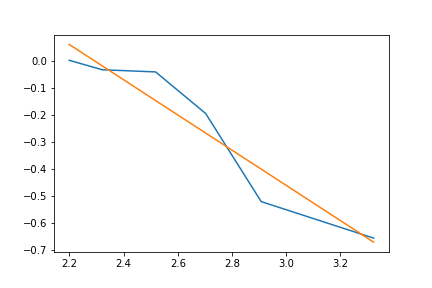
\includegraphics[width=0.6\linewidth]{./img/Fig.2.png}
    \caption{$U_g \sim \Delta L$}
    \label{fig:figure3}
\end{figure}
\begin{figure}[H]
    \centering
    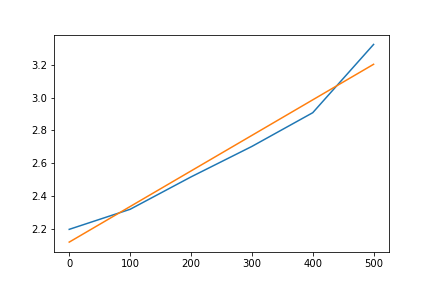
\includegraphics[width=0.6\linewidth]{./img/Fig.3.png}
    \caption{$\Delta L \sim \Delta m$}
    \label{fig:figure4}
\end{figure}
\end{document}